\section{Processos de Software}

Engenharia de Software pode ser definida como:
\begin{citacao}[english]
1. the systematic application of scientific and technological knowledge, methods, and experience to the design,
implementation, testing, and documentation of software [...]  2. the application
of a systematic, disciplined, quantifiable approach to the development, operation,
and maintenance of software; that is, the application of engineering to software \cite{IEEE2010}.
\end{citacao}

A engenharia de software deve ter foco na qualidade, que apoia as outras camadas
dessa tecnologia, que são as camadas de processo, métodos e ferramentas \autoref{fig:desen_engsoft}.
A camada de processo define um conjunto de atividades ou um arcabouço que tem
como finalidade garantir a efetiva utilização da tecnologia engenharia de software, que dessa forma
leva à produção de um software. Os detalhes de como fazer o software pertencem
a camada de métodos. Os métodos da engenharia de software incluem tarefas de planejamento
e estimativa de software, análise de requisitos, modelagem de projeto, codificação,
testes e manutenção. As ferramentas de engenharia de software auxiliam as camadas de
processo e métodos, com ferramentas automatizadas, que por sua vez, quando integradas,
é estabelecido um suporte ao desenvolvimento de software chamado CASE -
\textit{Computer Aided Software Engineering} \cite{Pressman2009, Sommerville2006}.

\begin{figure}[b]
  \centering
  \caption{Engenharia de Software - uma tecnologia em camadas}
  
\includegraphics[scale=0.3]{imagens/desenv_engsoft2}
  \label{fig:desen_engsoft}
  \fonte{\cite{Pressman2009}}
\end{figure}

Entre o conjunto de atividades definidas pela camada de processo, quatro são
fundamentais, a saber, especificação de software, projeto e implementação de
software, validação de software e evolução de software. Especificação de software
ou engenharia de requisitos é uma fase importante e crítica do processo de engenharia
de software. Importante porque é uma análise de requisitos bem feita que possibilitará
atendar as demandas dos usuários. Crítica porque um sistema mal especificado, pode até ser
bem projetado e construído, mas não vai atender as necessidades dos usuários.
Em seguida, na fase de projeto e implementação os requisitos são projetados e programados,
tendo como resultado um sistema executável. Depois, o software deve ser verificado
para mostrar que atende às demandas dos usuários (validação do software). Finalmente,
na fase de evolução de software, o mesmo é modificado devido às mudanças
de requisitos e às necessidades dos usuários.

% Quanto ao modelos de engenharia de software temos os modelos prescritivos e os ágeis.
% Os modelos prescritivos definem um conjunto de atividades explícitas para serem
% desenvolvidos no processo de engenharia de software. O Processo Unificado de desenvolvimento
% tem o maior destaque e reconhencimento dentre os modelos prescritivos.
%
% \subsection{Processo Unificado}
% O Processo Unificado define quatro atividades no processo de desenvolvimento de software.
% As fases são descritas como:
%
% \begin{description}
%   \item [{Concepção:}] Por meio da comunicação com os clientes, um conjunto
%   preliminar de casos de uso UML e da arquitetura do sistema é elaborada.
%   \item [{Elaboração:}] Nessa fase, os casos de uso UML são expandidos e
%   refinados, bem como a definição da arquitetura do sistema. Ao final
%   dessa fase, um conjunto de casos de uso UML descrevem os requisitos
%   dos sistema. Uma descrição da arquitetura do sistema e um plano de
%   desenvolvimento do software também são esperados.
%   \item [{Construção:}] Os casos de uso UML desenvolvidos na fase de elaboração
%   são então desenvolvidos e testados. O software deve estar funcionando
%   e documentado na conclusão dessa fase.
%   \item [{Transição:}] transferência do software aos usuários finais.
% \end{description}
%
% Fluxos de trabalhos ou \emph{workflows} ocorrem durante todas as
% fases no processo de desenvolvimento. São seis \emph{workflows} principais
% e três de apoio:
% \begin{enumerate}
%   \item \emph{Modelagem de negócios}: processos de negócios modelados por
%   casos de uso.
%   \item \emph{Requisitos}: atores são idenficados e casos de uso são desenvolvidos.
%   \item \emph{Análise e projeto: }vários modelos são desenvolvidos como de
%   arquitetura e componentes.
%   \item \emph{Implementação: }componentes são implementados.
%   \item \emph{Teste: }processo iterativo em conjunto com a implementação.
%   \item \emph{Implantação: }software é distribuído aos usuários finais.
%   \item \emph{Gerenciamento de configuração e mudança: }apoio as mudanças
%   do sistema.
%   \item \emph{Gerenciamento de projeto: }apoio de desenvolvimento do sistema.
%   \item \emph{Meio ambiente: }apoio a equipe de desenvolvimento com ferramentas.
% \end{enumerate}
%
\subsection{Métodos Ágeis}

Contrapondo-se aos modelos prescritivos em que propoem especificar por completo
os requisitos do sistema e só então projetar, construir e testar o sistema, surgiu
os métodos ágeis, que têm como filosofia o manifesto ágil \cite{Sommerville2006}.
Esse manifesto afirma \cite{agilemanifesto}:

\begin{citacao}
  Estamos descrobrindo melhores maneiras de desenvolver softwares, fazendo-o e ajudando
  outros a fazê-lo. Através dessse trabalho, valorizamos mais:\\\\
  \begin{minipage}{15cm}
    \begin{itemize}
      \item Indivíduos e interações do que processos e ferramentas
      \item Software em funcionamento do que documentação abrangente
      \item Colaboração do cliente do que negociação de contrato
      \item Resposta a mudanças do que seguir um plano
    \end{itemize}
  \end{minipage}\\\\
  Ou seja, embora itens à direita sejam importantes, valorizamos mais os que estão à esquerda.
\end{citacao}

Abordagens ágeis incluem \textit{Extreme Programming} e o \textit{Scrum}. Eles propõem diferentes processos
para que tenha-se um desenvolvimento e entrega incremental do sistema, tendo em comum princípios
baseados no manifesto ágil.

\section{Metodologias e Ferramentas}

A metodologia escolhida nesse projeto levou em consideração as necessidades de um trabalho de
conclusão de curso no curto prazo e os recursos limitados. Dessa forma, uma abordagem baseada em metodologias ágeis foi utilizada para %modelagem, documentação e codificação do software.
especificação, projeto e implementação do software. Nesse sentido, por exemplo,
na fase elicitação de requisitos não procurou-se a completa definição dos requisitos do software e ela nem foi
uma fase, a elaboração contínua dos requisitos fez parte do projeto de desenvolvimento como um todo.

% Práticas fundamentais implicam em aplicar os artefatos de modelagem corretos para cada situação, modelando o problema de forma incremental – sem a necessidade de criação de uma modelagem completa, irreal e fadada a ser, necessariamente, abandonada ou modificada posteriormente. Acredita-se ainda que os stakeholders do processo possuam o conhecimento sobre o que querem e podem prover tal conhecimento através de participação ativa, solicitada pelos modeladores.
%

\subsection{Objetivos específicos}

Para cada objetivo específico deste trabalho, as seguintes técnicas e ferramentas foram utilizadas:

\subsubsection{Realizar levantamento de requisitos sobre os sistemas de resposta em sala de aula}

A elicitação inicial de alto nível dos requisitos do sistema utilizou a análise de competidores que
consistiu basicamente em buscar em alguns sistemas de resposta existentes, referências positivas e
negativas para definição do modelo a ser proposto.

\subsubsection{Especificar e implementar uma aplicação web para o professor administrar as questões e gerar relatórios}
Os requisitos inicias gerados na análise de competidores, foram então transformados em tarefas, descritas
como histórias de usuário, com critérios de aceitação. A linguagem de programação usada na fase de implementação do aplicativo foi JavaScript, tendo como auxílio o \textit{framework} \textit{Ionic}.

\subsubsection{Especificar e implementar uma aplicação para dispositivos móveis, que será utilizado como {\clickers}}
Os requisitos inicias gerados na análise de competidores, foram então transformados em tarefas, descritas
como histórias de usuário, com critérios de aceitação. A linguagem de programação usada na fase de implementação do aplicativo foi JavaScript, tendo como auxílio o \textit{framework} \textit{Ionic}.

\subsubsection{Especificar e implementar um sistema servidor, para receber e
    enviar dados para os os clientes: dispositivos móveis dos alunos e navegador
    web do professor}

O sistema servidor foi desenvolvido utilizando tecnologias como \textit{Node.js}, \textit{MongoDB}, e o \textit{framework} \textit{FeathersJS}.
Tais tecnologias foram utilizadas por permitir o fácil desenvolvimento de aplicações web de tempo real entre o servidor e os seus clientes.

A teoria mais aprofundada sobre os métodos e ferramentas citadas serão descritas nas próximas seções.

\section{Especificação}

A fase inicial do projeto foi a de planejamento para a definição inicial de alto nível dos
requisitos do sistema. Nessa etapa, utilizou-se a análise de competidores para elucidar
os requisitos que posteriormente foram descritos como histórias de usuário.

\subsection{Análise de competidores}

A análise de competidores é uma técnica oriunda engenharia da usabilidade
que consiste em avaliar produtos concorrentes em busca de pontos positivos e
negativos. Tal técnica é útil no levantamento de requisitos de um novo sistema,
identificação de pontos fortes e fracos os produtos, reutilização de design, dentre outros \cite{nielsen_usability}.

Avaliar produtos concorrentes é valioso, porque oferece a oportunidade de novos
produtos evitarem problemas existentes dos competidores, explorar os pontos
fracos, além da reutilização dos pontos positivos \cite{nielsen_usability}.

Nesse sentido, a análise de competidores foi utilizada neste trabalho para elicitar requisitos e boas práticas
de design de interfaces. % bem como evitar problemos já identificados pelos concorrentes
Os resultados obtidos foram utilizados no desenvolvimento do software.

\subsubsection{\textit{Socrative}}

\textit{Socrative} é um sistema de resposta específico para usar em salas de aula. O sistema pode ser
acessado pelo site ou nos aplicativos para \textit{iOS} e \textit{Android}. No \textit{Socrative}, apenas o professor
precisa fazer um cadastro no site (questões demográficas são solicitadas). Existe uma versão
gratuita e paga do aplicativo.

Na conta do professor, é possível criar questionários de múltipla escolha, verdadeira e falso e
de questões abertas. Quando o professor cria uma conta, é gerado um código de identificação
para que os alunos possam entrar na sala virtual. Na interface do estudante, é necessário
colocar o código de identificação do professor.

\subsubsection{\textit{PollEverywhere}}

O \textit{PollEverywhere} é um sistema de resposta mais genérico, possibilitando fazer votações em
shows e apresentações diversas. Possibilita integração com ferramentas de apresentação
como o \textit{PowerPoint}. Outra característica é a possibilidade dos usuários votarem por SMS\nomenclature{SMS}{Short Message Service}.
Além dos tipos de questões básicas, o \textit{PollEverywhere} permite criar nuvem de palavras e
questões com imagens clicáveis.

A conta do usuário é associado com uma URL\nomenclature{URL}{Uniform Resource Locator}, em que é usada para os participantes
da votação entrarem e votarem.

\subsubsection{\textit{TopHat}}

\textit{TopHat} é outra solução voltada para a educação, contando com seis tipos de questões.
Adicionalmente o \textit{TopHat} permite ao professor fazer a chamada dos estudantes, isso porque
o professor pode gerar um código aleatório no \textit{TopHat} para que os estudantes presentes
possam enviar o código e marcar presença. O produto também disponibiliza uma sala
de discussão e a possibilidade de criar slides dentro do aplicativo.

\begin{center}
\begin{table}
\caption{Análise de Competidores}
\begin{centering}
\begin{tabular}{>{\centering}m{4cm}||>{\centering}p{4cm}>{\centering}p{3.5cm}c}
\hline
\multicolumn{1}{>{\centering}m{3.5cm}}{Caraterística} & \textit{PollEverywhere} & \textit{TopHat} & \textit{Socrative}\tabularnewline
\hline
\hline
Open-Source & Não & Não & Não\tabularnewline
Integração com LMS & Blackboard & Excel & MasteryConnect\tabularnewline
Formatos & JSON, RSS, CSV & Não & Não\tabularnewline
Read-only API & Sim & Não & Não\tabularnewline
Integração com PowerPoint & Possibilita & Não & Não\tabularnewline
Métodos de votação & SMS, web & SMS, Web & Internet\tabularnewline
Tempo-real & Sim & Sim & Sim\tabularnewline
Acesso ao sistema & URL & Código de Acesso & Código de Acesso\tabularnewline
Tipos de questões & 5 & 7 & 3\tabularnewline
Mínimo de passos para votação & 2 & 3 & 4\tabularnewline
Anonimato & Possibilita & Possibilita & Possibilita\tabularnewline
Contagem regressiva & Possibilita & Possibilita & Não\tabularnewline
Download CSV & Possibilita & Não & Não\tabularnewline
Relatórios por estudante & Possibilita & Possibilita & Não\tabularnewline
\hline
\end{tabular}
\par\end{centering}

\doautor
\end{table}

\par\end{center}

\subsection{Requisitos gerados a partir da análise de competidores}\label{sec:requisitos}

A partir das informações coletadas na análise de competidores, foram
extraídos um conjunto de requisitos iniciais para o sistema. Os requisitos
funcionais gerados pela análise dos competidores foram então descritos como histórias de usuário.
A seguir descreve-se os requisitos gerados:

\begin{description}
\item[Integração com sistemas LMS\nomenclature{LMS}{Learning Management System}]: O sistema deve permitir integração com
sistemas LMS (Amadeus, Moodle);
\item[Todas as plataformas:] é muito importante que o sistema seja capaz
de funcionar em smartphones, tables e computadores independentemente
do sistema operacional.
\item[Questões abertas, verdadeiro/falso e de múltipla-escolha:] O sistema
deve fornecer pelo menos esses três tipos básico de questões;
\item[Modo de votação:] O sistema deve permitir votação anonima ou requisitar
a identificação;
\item[Customização das questões:] O sistema deve permitir inserção de equações
matemáticas (\LaTeX), imagens e texto como opção das questões;
\item[Controle da votação:] Opções básicas como ativar ou desativar a votação
e limpar uma votação em andamento;
\item[Controle de frequência:] o sistema gera um código aleatório ou uma
questão trivial, em que o professor pode solicitar que os estudantes
respondam, contando como controle de frequência. Os dados devem ser
facilmente exportados para CSV\nomenclature{CSV}{Comma-separated values}.
\item[Tempo-real:] No momento da votação, o professor pode escolher entre
apresentar o resultado em tempo-real, quando todos votarem, ou quando
determinado;
\item[Banco de questões:] As questões elaboradas pelo professor podem ser
armazenadas em um banco de questões que o sistema deve manter;
\item[Facilidade do uso e de criação de votação:] O sistema não deve oferecer
dificuldades de uso e de criação de questões;
\item[Código de acesso:] O sistema deve gerar um código de acesso único para
identificar o ambiente do professor, usado para que os alunos respondam.
\end{description}

\subsection{Histórias de Usuário}

A metodologia ágil de software, \textit{eXtreme Programming (XP)}, introduziu a
prática de expressar os requisitos de software na forma de \textit{histórias de usuário},
que são descricões informais do que  o sistema deve fazer, evitando qualquer terminologia técnica \cite{Sommerville2006}.

As histórias de usuário (\autoref{fig:backlog}), formaram a lista de tarefas do projeto. Essa
lista de tarefas foi então priorizada, de forma que, por exemplo, desenvolver a arquitetura
que possibilita-se ao professor apresentar uma questão no quadro e habilitar para os alunos
responderem foi a primeira tarefa a ser desenvolvida. Por outro lado, a tarefa de permitir
categorizar as questões para permitir um agrupamento de questões teve uma prioridade baixa.

\begin{figure}[!ht]
  \centering

  \caption{Requisitos iniciais para o sistema em forma de histórias de usuário}
  \subfloat{
    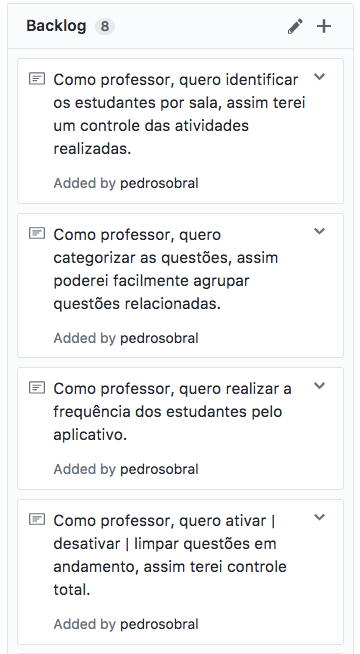
\includegraphics[scale=0.65,valign=t]{imagens/backlog1.png}
  }
  \subfloat{
    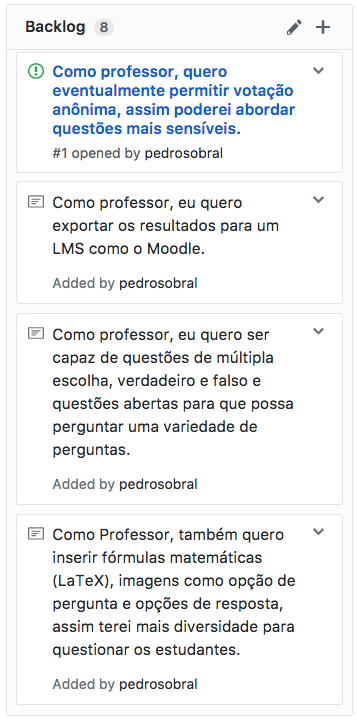
\includegraphics[scale=0.65,valign=t]{imagens/backlog2.png}
  }
  \doautor
  \label{fig:backlog}
\end{figure}


\section{Projeto e Implementação}

\subsection{Plataforma}

\begin{description}
  \item[JavaScript:] é uma linguagem de programação leve, interpretada e orientada a objetos com funções de primeira classe
  (funções no JavaScript podem ser passadas como argumento para outras funções, pode ser o valor retornado por outras funções e ainda
  podem ser atribuídas para variáveis).
  Ela é uma linguagem de scripting baseada em protótipos, multi-paradigma e dinâmica, suportando os estilos orientado a objetos, imperativo e funcional.
  Uma das implementações ou \textit{engine} mais populares de JavaScript é o V8 da Google que
  é utilizada pelo navegador Google Chrome e também pelo Opera \cite{javascript}.
  \item[Node.js:] é uma plataforma construída sobre o \textit{engine} V8 da Google
  para construir aplicações de rede rápidas e escaláveis. Node.js usa um modelo de I/O direcionada a
  evento não bloqueante que o torna leve e eficiente, ideal para aplicações em
  tempo real com troca intensa de dados através de dispositivos distribuídos \cite{nodejs}.
  \item[MongoDB:] é um sistema de gerenciamento de banco de dados orientado à documentos.
  Ele é classificado como um banco de dados \textit{NoSQL}, ou seja, o mecanismo de
  armazenamento e recuperação é modelado de outras formas além da forma relacional. O MongoDB  usa o modelo de
  dados JSON para mapear as aplicações de forma simples e rápida \cite{mongodb}.
\end{description}

\subsection{Arquitetura}

A \autoref{fig:arquitetura} exibe a arquitetura do sistema. Ela consiste dos clientes (aplicação professor e aplicativo dos alunos), e do servidor
desenvolvido na plataforma Node.js com o \textit{framework}
\textit{FeathersJS} que recebe as requisições dos clientes.
A comunicação entre o nó cliente e o nó servidor é por
meio do protocolo \textit{WebSocket}. O servidor faz a interface com o banco de
dados MongoDB.

\begin{figure}[!ht]
  \centering

  \caption{Arquitetura do sistema}
  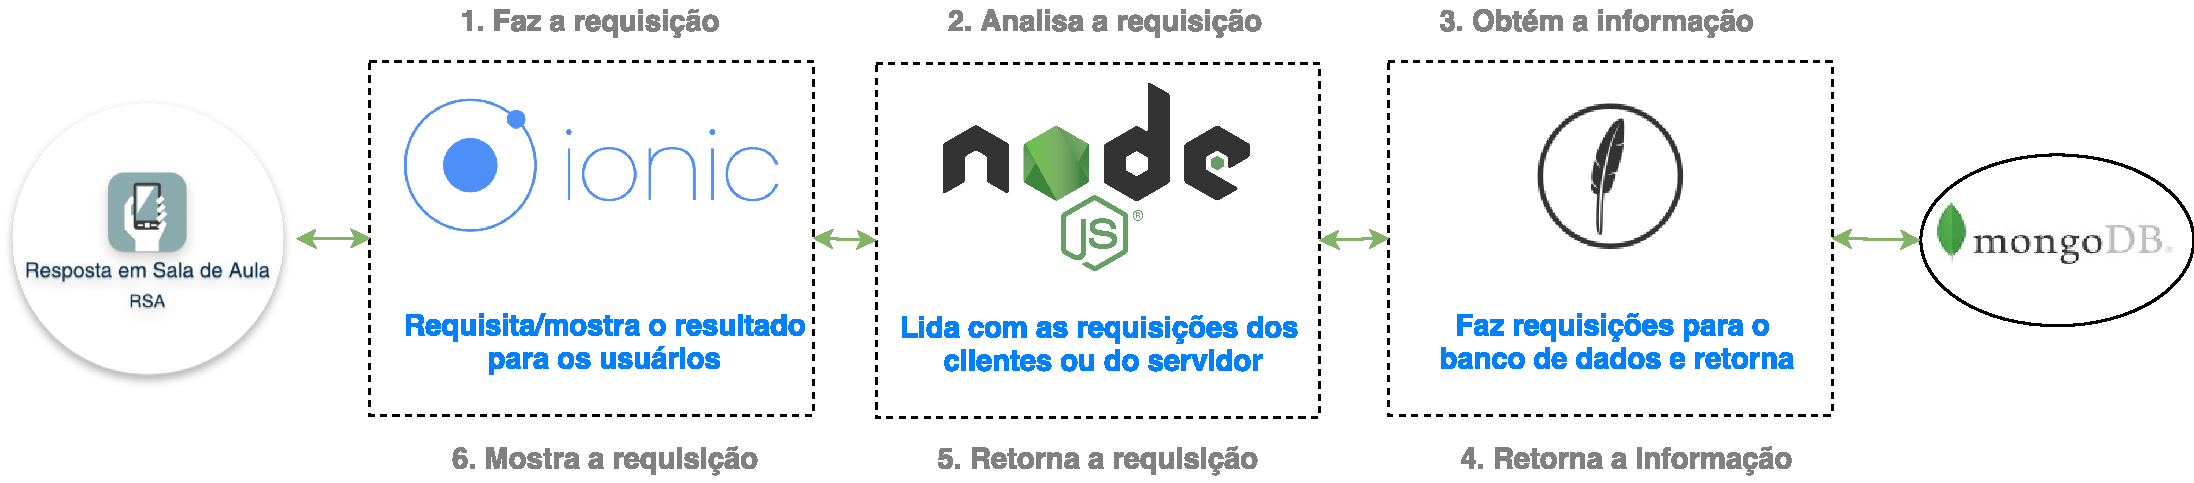
\includegraphics[scale=.45]{imagens/arquitetura.pdf}
  \label{fig:arquitetura}
  \doautor

\end{figure}

\subsection{\textit{WebSocket} para aplicações em tempo real}

\textit{WebSocket} é um protocolo que possibilita abrir um canal interativo de comunicação
entre o navegador e o servidor. Na verdade, esse canal é bidirecional (\textit{full-duplex})
que utiliza apenas um soquete TCP\nomenclature{TCP}{Transmission Control Protocol} \cite{websocket2016}.
A tecnologia \textit{WebSocket} foi usada para permitir votação e controle de frequência em tempo-real.

\subsection{Estrutura do Framework: \textit{Ionic}}

\textit{Ionic} é um \textit{framework open-source} para o desenvolvimento de aplicativos
híbridos utilizando tecnologias web como HTML\nomenclature{HTML}{HyperText Markup Language},
CSS\nomenclature{CSS}{Cascading Style Sheets} e JavaScript otimizadas
para dispositivos móveis, com código fonte sobre a licença MIT\nomenclature{MIT}{Massachusetts Institute of Technology} \cite{ionic2016}.
Uma das principais vantagens do desenvolvimento de aplicativos híbridos é que com
apenas um código base é possível criar aplicativos para várias plataformas como
\textit{iOS}, \textit{Android} e \textit{Windows} Phone, Desktop, que aliás foi uma das razões que fez o Moodle
usar o \textit{Ionic} como \textit{framework} para o desenvolvimento do \textit{Moodle Mobile 2} \cite{moodle2016}.

\subsubsection{Pages}

Um aplicativo desenvolvido no \textit{Ionic} é composto por um conjunto de pages ou páginas.
Cada página é composta por alguns arquivos. Um arquivo é responsável pelo
elemento visual da página, desenvolvido em HTML. Existe o arquivo de estilos da página,
desenvolvido em CSS. O arquivo principal é o responsável por controlar a página, desenvolvido
em TypeScript.

As Figuras \ref{fig:hello_ionic_ts} e \ref{fig:hello_ionic_html} são um exemplo básico de
uma página de um aplicativo desenvolvido em \textit{Ionic}. O resultado dessa página é mostrado
na \autoref{fig:hello_world_ionic}. Observe que com apenas um código base, os elementos
visuais da página são diferentes dependendo da plataforma (\textit{iOS}, \textit{Android} e \textit{Windows}).

\begin{figure}[ht]
\begin{lstlisting}[language=JavaScript]
  import { Component } from '@angular/core';

  @Component({
    selector: 'page-hello-ionic',
    templateUrl: 'hello-ionic.html'
  })
  export class HelloIonicPage {
    constructor() {}
  }
\end{lstlisting}
\caption{HelloIonicPage: classe responsável por exibir e controlar a página}
\label{fig:hello_ionic_ts}
\end{figure}

\begin{figure}[ht]
\caption{HelloIonicPage: elementos visuais da página}
\begin{lstlisting}[language=ionicHtml]
  <ion-header>
    <ion-navbar>
      <button ion-button menuToggle>
        <ion-icon name='menu'></ion-icon>
      </button>
      <ion-title>Hello Ionic</ion-title>
    </ion-navbar>
  </ion-header>

  <ion-content padding>

    <h3>Welcome to your first Ionic app!</h3>

    <p>
      This starter project is our way of helping you get a functional app running in record time.
    </p>
    <p>
      Follow along on the tutorial section of the Ionic docs!
    </p>
    <p>
      <button ion-button color='primary' menuToggle>Toggle Menu</button>
    </p>

  </ion-content>
\end{lstlisting}
\doautor
\label{fig:hello_ionic_html}
\end{figure}

\begin{figure}[ht]
  \centering
  \caption{Página em \textit{Ionic} resultado  das Figuras \ref{fig:hello_ionic_ts} e \ref{fig:hello_ionic_html}}
  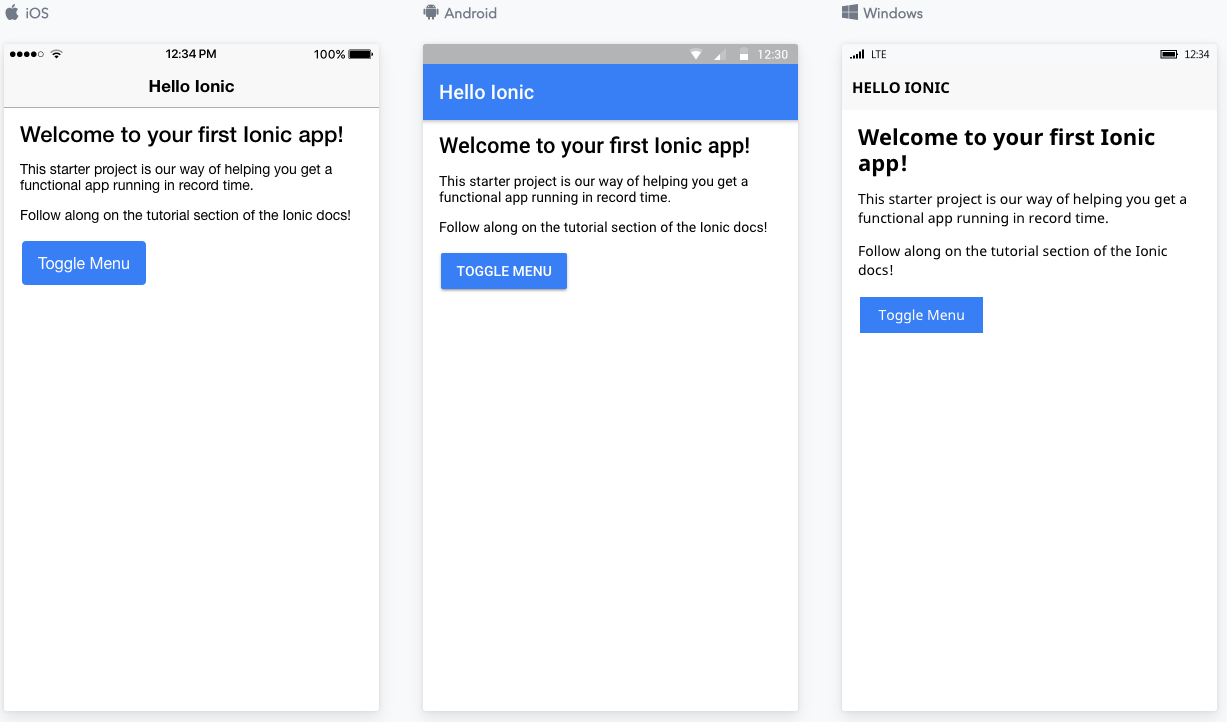
\includegraphics[scale=.34]{imagens/hello_world_ionic.png}
  \doautor
  \label{fig:hello_world_ionic}
\end{figure}

\subsubsection{Components}

Os elementos visuais e também o comportamento desses elementos em uma página
são normalmente construídos por meio dos \textit{components} ou componentes.
Os componentes permitem criar facilmente a interface do aplicativo. Exemplo de
componentes são botões, \textit{modals, popup} e \textit{cards}. Um aspecto interessante é que
os componentes se adaptam visualmente a cada plataforma, como já mostramos na \autoref{fig:hello_world_ionic}.
Além do aspecto visual eles também se comportam de maneira diferente dependendo da plataforma.
Por comportamento, entende-se, por exemplo, os efeitos visuais de cada componente e também efeitos
de  transição entre as páginas. A \autoref{fig:ionic_components} ilustra alguns componentes
disponíveis no \textit{Ionic}.

\begin{figure}
  \centering

  \caption{Exemplo de componentes no \textit{Ionic}}
  \label{fig:ionic_components}
  \subfloat[List]{
    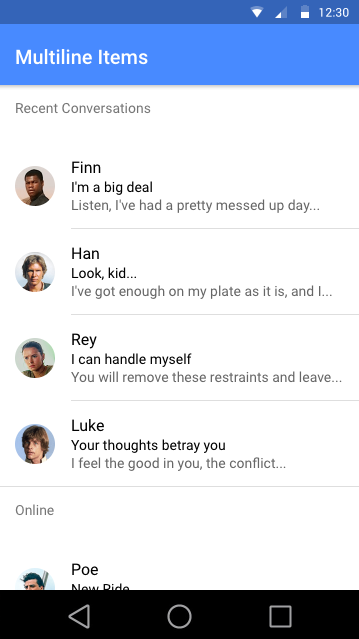
\includegraphics[scale=0.3,valign=t]{imagens/cmp1.png}
  }
  \subfloat[DateTime]{
    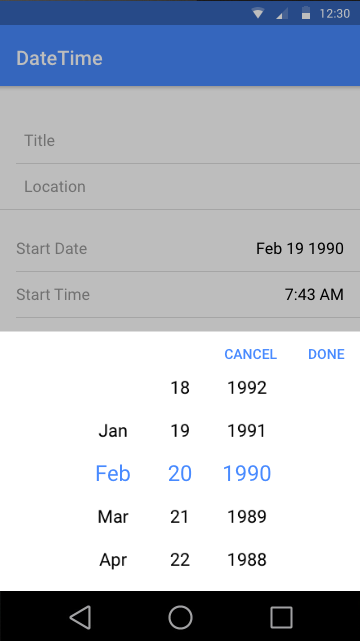
\includegraphics[scale=0.3,valign=t]{imagens/cmp2.png}
  }

  \subfloat[Float Action Buttons]{
    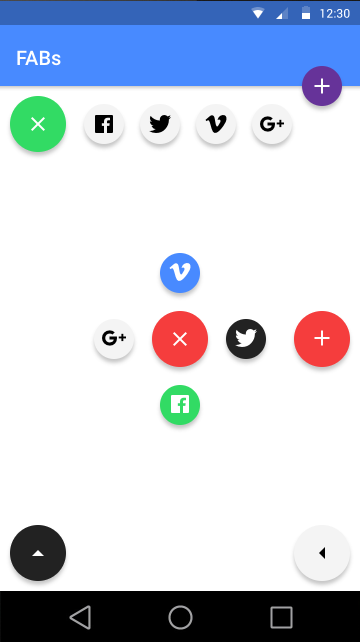
\includegraphics[scale=0.3,valign=t]{imagens/cmp3.png}
  }
  \subfloat[Menu]{
    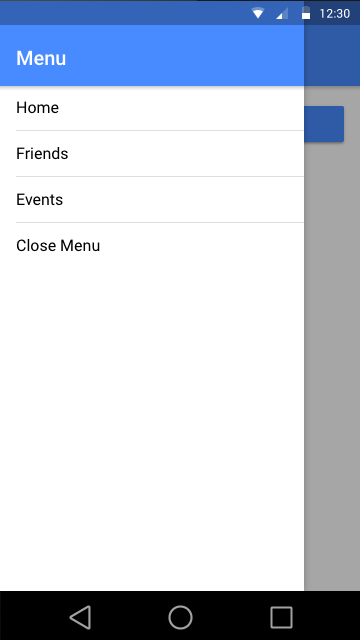
\includegraphics[scale=0.3,valign=t]{imagens/cmp4.png}
  }

  \subfloat[Checkboxes]{
    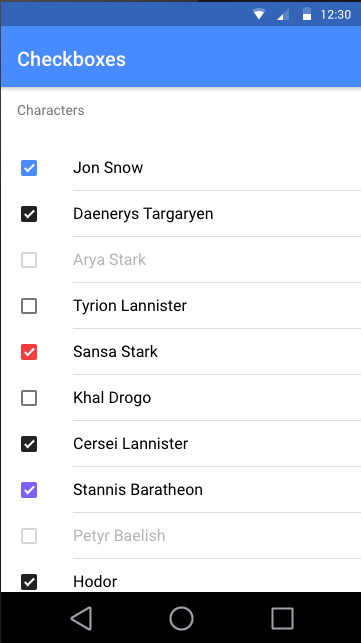
\includegraphics[scale=0.3,valign=t]{imagens/cmp5.png}
  }
  \subfloat[Action Sheets]{
    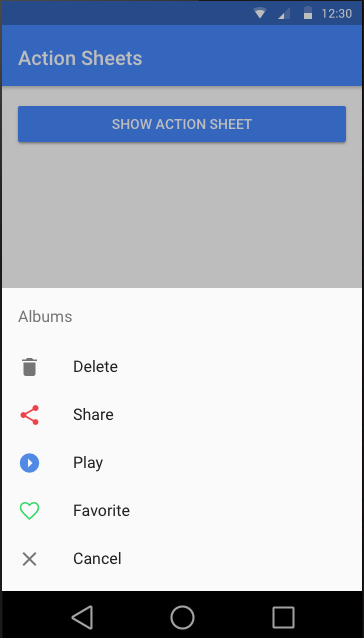
\includegraphics[scale=0.3,valign=t]{imagens/cmp6.png}
  }
  \fonte{Disponível em: \href{http://ionicframework.com/docs/components}{http://ionicframework.com/docs/components/}. Acesso em 28 Mai. 2017}
\end{figure}

\clearpage
\subsection{Estrutura do Framework: \textit{FeathersJS}}

\textit{FeathersJS} é um \textit{framework open-source} de desenvolvimento rápido para aplicações
web em tempo-real escritas em JavaScript. Disponibiliza uma arquitetura simples mas poderosa
para a construção de aplicações utilizando padrões de programação orientada a aspectos e serviços \cite{feathers}.
Os principais componentes do \textit{FeathersJS} são os \textit{services}, \textit{hooks} e
\textit{events} que são detalhados nas próximas seções.

\subsubsection{Services}\label{subsection:feathers_services}
\textit{Services} ou serviços são a camada principal do \textit{\textit{FeathersJS}}.
Um serviço é simplesmente uma instância de uma classe JavaScript
que implementa métodos básicos para criação, consulta, atualização e
destruição de dados. Esse conjunto de operações ou funcionalidades é conhecido como
CRUD (\textit{Create, Read, Update, Delete}).

Os serviços no \textit{FeathersJS} expõem uma interface uniforme de acesso, permitindo
assim fornecer uma única API\nomenclature{API}{Application Programming Interface} tanto para chamadas
HTTP\nomenclature{HTTP}{Hypertext Transfer Protocol} REST\nomenclature{REST}{Representational State Transfer} e \textit{websockets}.
Os verbos HTTP (GET, POST, PUT, PATCH e DELETE) têm a correspondência com
os métodos de um serviço no \textit{\textit{FeathersJS}} listados na \autoref{fig:service_interface}.

\begin{figure}[h]
\caption{Interface de um serviço}
\label{fig:service_interface}
\begin{lstlisting}[language=JavaScript]
const meuServico = {
  // GET /path
  find(params, callback) {},
  // GET /path/<id>
  get(id, params, callback) {},
  // POST /path
  create(data, params, callback) {},
  // PUT /path/<id>
  update(id, data, params, callback) {},
  // PATCH /path/<id>
  patch(id, data, params, callback) {},
  // DELETE /path/<id>
  remove(id, params, callback) {}
}
\end{lstlisting}
\doautor
\end{figure}

\subsubsection{Hooks}

\textit{Hooks} são técnicamente \textit{middleware} ou funções que têm acesso aos
objetos de solicitação (\texttt{req}) e resposta (\texttt{res}).
Dessa forma os \textit{hooks} podem fazer mudanças nos objetos de solicitação e resposta.
O \textit{\textit{FeathersJS}} permite registrar \textit{hooks} antes (\textit{before}), depois
(\textit{after}) ou em caso de erro (\textit{error}) dos métodos de
um serviço, como mostrado na \autoref{fig:service_interface}.

Como eles têm acesso ao objetos de uma requisição (\texttt{req} e \texttt{res}), eles são usados
para política de controle de acesso da aplicação, registro de eventos, enviar
notificações, adicionar propriedades e muito mais.

Essa abordagem é conhecida como Programação Orientada a Aspectos, que permite
a separação de propriedades ortogonais (ou que não fazem parte da funcionalidade
principal) dos componentes funcionais de uma forma natural e concisa.

Na \autoref{fig:hooks_example} três \textit{hooks} foram registrados para um serviço de questões (\textit{questions}) ($\ell.\,1$),
em que é adicionado a propriedade \texttt{createdAt} antes (\textit{before}) da criação (\textit{create}) de um objeto questão ($\ell.\,3-5$),
e a propriedade \texttt{updatedAt} quando uma questão é modificada (\textit{update} e \textit{patch}), ($\ell.\,7-13$).

\begin{figure}[h]
\caption{Exemplo registro de \textit{hooks} no \textit{\textit{FeathersJS}}}
\label{fig:hooks_example}
\begin{lstlisting}[language=JavaScript]
  app.service('questions').hooks({
    before: {
        create(hook) {
          hook.data.createdAt = new Date();
        },

        update(hook) {
          hook.data.updatedAt = new Date();
        },

        patch(hook) {
          hook.data.updatedAt = new Date();
        }
      }
  });
\end{lstlisting}
\doautor
\end{figure}

\subsubsection{Events}

São os \textit{events} ou eventos no \textit{\textit{FeathersJS}} permitem
a criação de aplicações de tempo-real usando \textit{WebSockets}.

No \textit{\textit{FeathersJS}}, os serviços enviam automaticamente eventos ou notificações
\texttt{created, updated, patched, removed} quando algum dos respectivos métodos listados
na \autoref{fig:service_interface} finalizam com sucesso.
Os clientes da aplicação podem então ouvir a esses eventos e reagirem de acordo.

Na \autoref{fig:events_example} o cliente obtém uma referência do serviço
de votação ($\ell.\,2$) e então passa a ouvir quando uma nova votação é criada (\texttt{created}) ($\ell.\,5-7$).
Nesse caso, os clientes de uma aplicação de votação, por exemplo, poderiam
receber as questões da votação publicada por outro cliente e então responder.

\begin{figure}[h]
\caption{Exemplo eventos no \textit{\textit{FeathersJS}}}
\label{fig:events_example}
\begin{lstlisting}[language=JavaScript]
  // Retrieve the wrapped service object which will be an event emitter
  const poll = app.service('poll');

  // Listen `created` event
  poll.on('created', (poll) => {
    console.log('New poll created', poll);
  });
\end{lstlisting}
\doautor
\end{figure}

\subsubsection{Visão geral}

A \autoref{fig:feathers_request} ilustra como funciona o ciclo de uma requisição
entre clientes e uma aplicação baseada no \textit{FeathersJS}.

O cliente faz uma requisição para um serviço, que antes de chegar no serviço passa
pela camada de \textit{before hooks}, o método requisitado pode completar com sucesso indo para a
\textit{after hooks} e enviando um evento para os clientes conectados. Qualquer erro no processo
é enviado para a camada \textit{error hooks} que também pode notificar os clientes da aplicação.

\begin{figure}[!ht]
  \centering
  \caption{Como o ciclo de uma requisição funciona no \textit{FeathersJS}}
  \label{fig:feathers_request}
  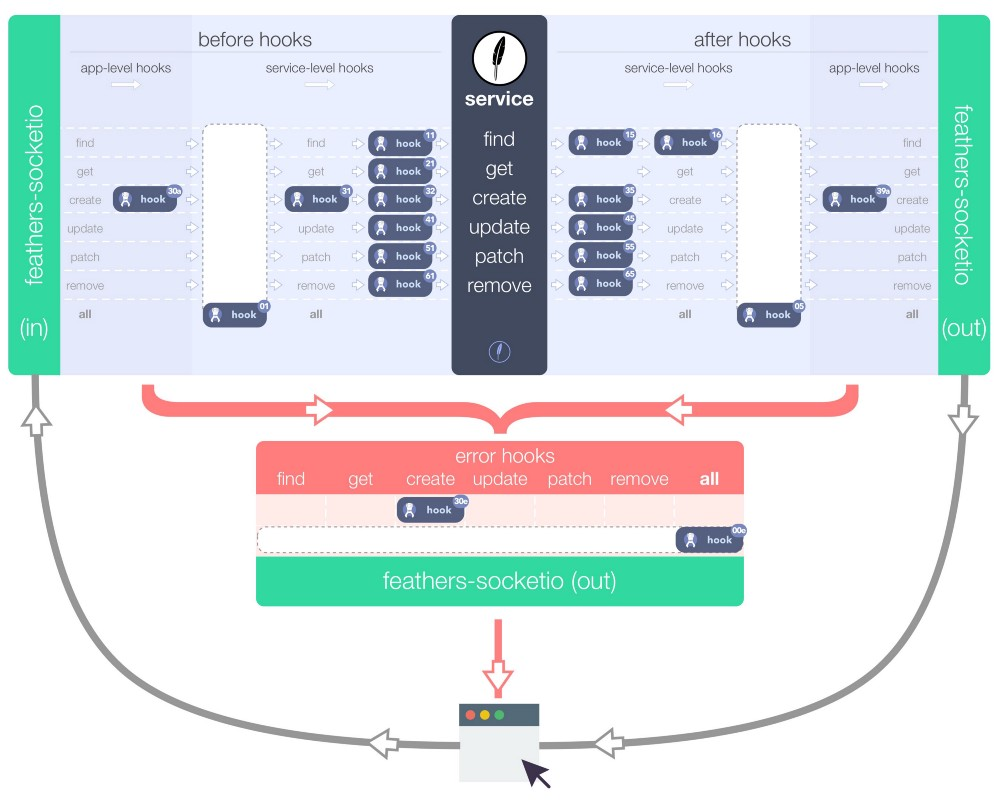
\includegraphics[scale=0.4,valign=t]{imagens/feathers_request.jpeg}
  \fonte{Disponível em: \href{https://docs.feathersjs.com/guides/step-by-step/basic-feathers/all-about-hooks.html}{docs.feathersjs.com/guides/step-by-step/basic-feathers/all-about-hooks.html}. Acesso em 29 Mai. 2017}
\end{figure}

A utilização do \textit{FeathersJS} simplificou muito o processo de construção
do software por disponibilizar facilidades para o programador e implementar
uma API de tempo-real via serviços de forma nativa. Além disso, a interface dos
serviços \autoref{fig:service_interface} torna fácil a integração com qualquer banco de dados.
Nesse sentido, o \textit{FeathersJS} suporta alguns ORM que permitem uma integração
com uma variedade de banco de dados por meio de uma interface única.

% \clearpage
\subsection{Implementação}\label{subsection:implementation}

Os items da lista de tarefas da \autoref{fig:backlog} foram desenvolvidos de forma incremental.
Para cada história de usuário desenvolvida, procurava-se desenvolver os critérios de aceitação da mesma.
Os critérios de aceitação geralmente definem o comportamento esperado da funcionalidade desenvolvida pela história.
Dessa forma, eles são úteis para definir quando uma história foi finalizada e implementada de forma correta.

Os critérios de aceitção foram escritos usando o formato utilizado no desenvolvimento dirigido por
comportamento (\textit{Behavior-Driven Development (BDD)}\nomenclature{BDD}{Behavior-Driven Development}).
No BDD descreve-se o comportamento no seguinte formato:

\begin{description}
  \item[Dado que (\textit{Given}):] determinadas pré-condições são atendidadas;
  \item[Quando (\textit{When}):] um determinado evento ocorre;
  \item[Então (\textit{Then}):] isso deve acontecer.
\end{description}
Considere por exemplo, a história de usuário:
\begin{description}
  \item[Como] professor
  \item[Gostaria] ser capaz de criar (questões de múltipla escolha | verdadeiro e falso | questões abertas)
  \item[para] que eu tenha variedade de perguntas para explorar.
\end{description}
Tem-se os seguintes critérios de aceitação:
\begin{enumerate}
  \item
  \begin{description}
    \item[Dado que] o professor pode criar uma questão
    \item[Quando] ele escolher criar uma questão do tipo múltipla escolha
    \item[E] preencher o campo \textit{questão}
    \item[E] adicionar pelo menos duas alternativas
    \item[E] escolher uma alternativa como a correta
    \item[E] clicar no botão \textit{CONCLUÍDO}
    \item[Então] o sistema deve permitir salvar a questão
    \item[E] indicar que a questão foi salva com sucesso
    \item[E] eu devo ser redirecionado para a aba \textit{Questões}.
  \end{description}

  \item
  \begin{description}
    \item[Dado que] o professor pode criar uma questão
    \item[Quando] ele escolher criar uma questão do tipo múltipla escolha
    \item[E] preencher o campo \textit{questão}
    \item[E] não adicionar pelo menos duas alternativas
    \item[E] não escolher uma alternativa como a correta
    \item[Então] o sistema não deve permitir salvar a questão
    \item[E] indicar que é necessário adicionar pelo menos duas alternativas
    \item[E] indicar que é necessário escolher uma alternativa como a correta.
  \end{description}
\end{enumerate}

\subsubsection{Banco de Dados: MongoDB}

O banco de dados utilizado foi o MongoDB que é um banco de dados NoSQL orientado a documentos.
Em tais bancos os dados são \textit{semiestruturados}. Dados semiestruturados
são dados em que o esquema de representação está presente em conjunto com o dado, ou seja,
eles são \textit{auto-descritivos}. As nomenclaturas do MongoDB diferem dos
bancos relacionais. A \autoref{tab:relvsmongo} apresenta como eles se relacionam.

\begin{table}[!ht]
  \centering
  \caption{Nomenclaturas dos banco de dados relacionais $versus$ MongoDB}
  \begin{tabular}{l||l}
    \hline
    \textbf{Banco Relacional} & \textbf{MongoDB}\tabularnewline
    \hline
    \hline
    Base de dados & Base de dados\tabularnewline
    Tabela & Coleção\tabularnewline
    Registro & Documento\tabularnewline
    Coluna & Campo\tabularnewline
    Índice & Índice\tabularnewline
    Join & Documento Embarcado\tabularnewline
    Chave estrangeira & Referência\tabularnewline
    \hline
  \end{tabular}
  \doautor
  \label{tab:relvsmongo}
\end{table}

O MongoDB armazena os dados no formato chamado BJSON (Binary JSON). O BJSON extende
o JSON\nomenclature{JSON}{JavaScript Object Notation} (JavaScript Object Notation) incluindo suporte para tipos de dados
\texttt{int, long, date, floating point} e \texttt{decimal128}. Um documento BJSON\nomenclature{BJSON}{Binary JavaScript Object Notation} contem
um ou mais campos, e cada campo um valor de um tipo específico, incluíndo vetores, dados
binários, e outros sub-documentos \cite{mongodb}. A \autoref{fig:mongodocument} apresenta um
exemplo de um documento em MongoDB.

Documentos (ou \textit{documents}) que tendem a compartilhar a mesma estrutura
são organizados como \textit{coleções} (ou \textit{collections}). Coleções são
análogas a uma tabela em um banco de dados relacional, documentos são similares
a registros ou linhas, e campos são parecidos com as colunas.

\begin{figure}[ht]
  \caption{Exemplo de um documento em MongoDB}
  \label{fig:mongodocument}
  \begin{lstlisting}[language=JavaScript]
  {
  	"_id" : ObjectId("59526b5801f55103c054779c"),
  	"name" : "Engenharia de Software",
  	"code" : "ENGSOFT123",
  	"user" : ObjectId("59526b2001f55103c054779b"),
  	"updatedAt" : ISODate("2017-06-27T14:27:36.113Z"),
  	"createdAt" : ISODate("2017-06-27T14:27:36.113Z"),
  	"peopleOnline" : -2,
  	"private" : true,
  	"online" : true,
  	"students" : [
  		{
  			"_id" : ObjectId("59526b7601f55103c054779e"),
  			"online" : false,
  			"id" : "102",
  			"name" : "Paulo"
  		},
  		{
  			"_id" : ObjectId("59526b7601f55103c054779d"),
  			"online" : false,
  			"id" : "101",
  			"name" : "Pedro"
  		}
  	],
  	"__v" : 0
  }
  \end{lstlisting}
  \doautor
\end{figure}

A \autoref{fig:database} exibe uma versão simplificada de como os dados
foram estruturados. O sistema tem basicamente quatro coleções:
\textit{User (Usuário), Poll (votação), Room (Sala), Attendance (Frequência), Question (Questão)}.
Nesse esquema, as questões (\textit{question}) são sub-documentos dentro de uma votação (\textit{poll}), dessa forma,
com apenas uma leitura no banco de dados é possível obter toda a informação de uma votação.

\begin{figure}[!ht]
  \centering
  \caption{Diagrama do banco de dados orientado a documentos}
  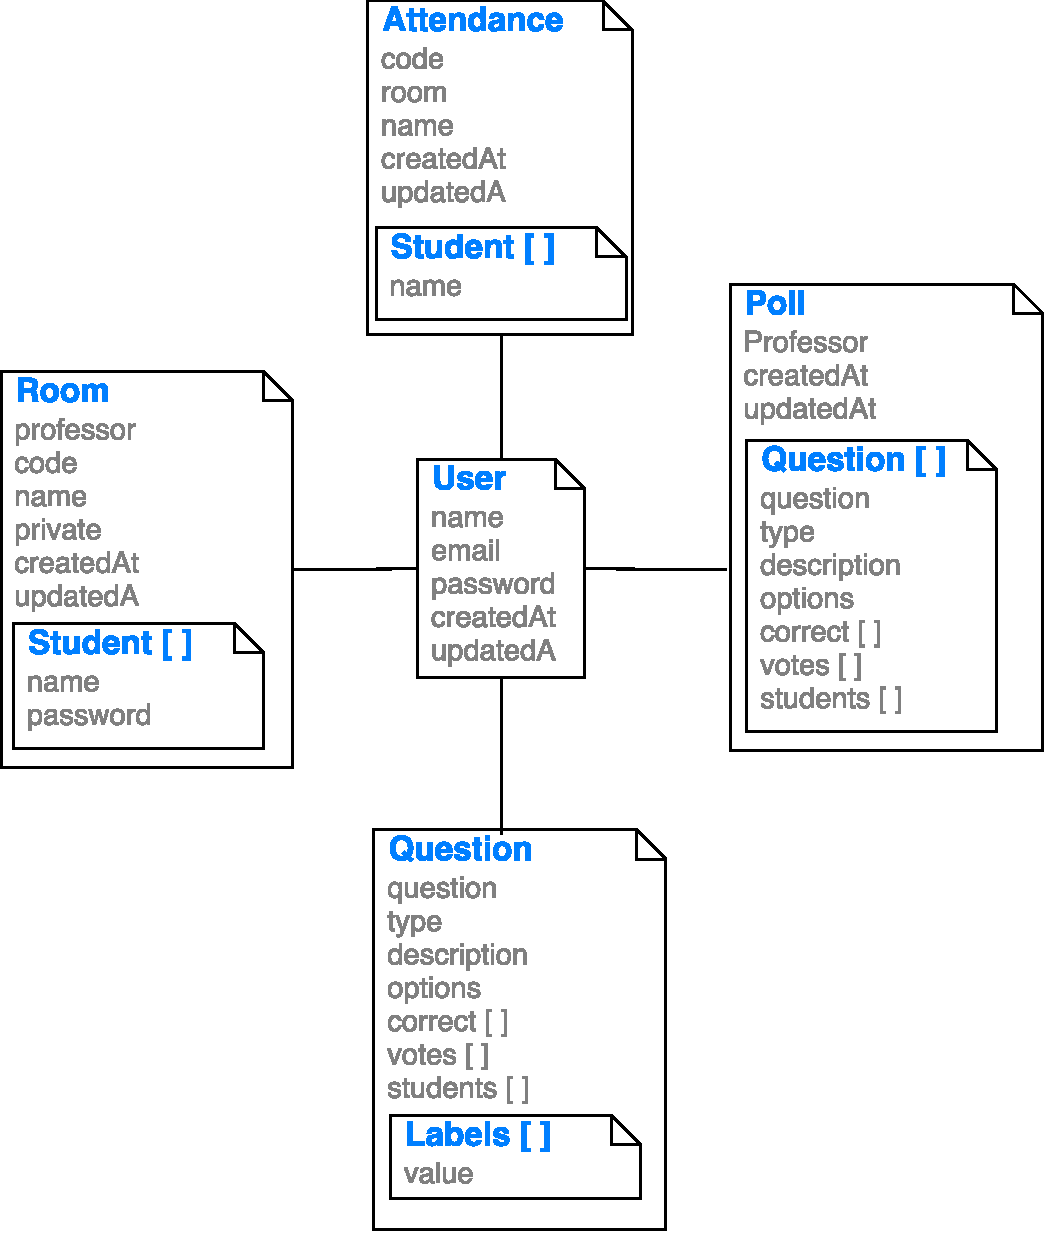
\includegraphics[scale=0.75,valign=t]{imagens/database}
  \doautor
  \label{fig:database}
\end{figure}

\subsection{Servidor: FeathersJS}

O principal componente de uma aplicação desenvolvida com o \textit{FeathersJS} são os
serviços. Os serviços foram explicados em detalhes na \autoref{subsection:feathers_services}.

Para cada coleção do banco de dados mostrado na \autoref{fig:database} foi desenvolvido um
serviço correspondente no \textit{FeathersJS}. Para auxiliar nesse processo, o \textit{FeathersJS} conta com
uma ferramenta para tornar ainda mais rápido o processo de desenvolvimento de aplicações.
Um deles é o utilitário de linha de comando \texttt{feathers} capaz de gerar
os principais componentes do \textit{framework} como os \textit{services} e \textit{hooks}.

A \autoref{fig:feathers_generate} ilustra a utilização da ferramenta para a geração do serviço
\textit{question} do tipo \textit{MongoDB}. Nesse exemplo, como o serviço é do tipo MongoDB, ao
final do processo tem-se uma REST API totalmente funcional, por não ser preciso definir um modelo do serviço.
Se um banco de dados relacional fosse usado como o tipo do serviço, teria-se que desenvolver o modelo do esquema da tabela primeiro.

\begin{figure}[!ht]
  \centering
  \caption{Interface de linha de comando da ferramenta \texttt{feathers}}
  \label{fig:feathers_generate}
  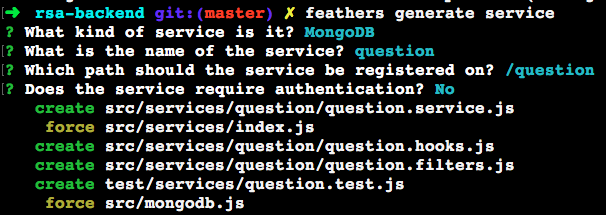
\includegraphics[scale=0.6,valign=t]{imagens/feathers_generate}
  \doautor
\end{figure}

\subsection{Frontend: Ionic}

Uma das características interessantes do FeathersJS é que ele também funciona
como cliente no navegador exatamente da mesma forma como no servidor.
A \autoref{fig:feathers_provider}, mostra um serviço que faz parte da aplicação web desenvolvida em Ionic,
que é responsável por obter as informações nesse caso específico \textit{Poll (votação)}.

Na ($\ell.\,2$) importa-se a classe responsável por fazer a conexão com o servidor e que também
expõem alguns métodos como por exemplo para obter uma referência de um serviço do servidor ($\ell.\,6$). Na ($\ell.\,11-13$)
tem-se o método para criar uma votação. Na ($\ell.\,16-23$), o método \texttt{poll(room)} retorna uma votação
que tenha um código específico de uma sala ($\ell.\,19$) e que não ainda não tenha sido encerrada ($\ell.\,20$).

\begin{figure}[!ht]
  \caption{\textit{PollService} - serviço para prover informações do serviço de votações}
  \label{fig:feathers_provider}
  \begin{lstlisting}[language=JavaScript]
    import { Injectable } from '@angular/core';
    import { FeathersProvider } from './feathers';

    @Injectable()
    export class PollService {
      polls = this.app.service('polls');

      constructor(public app: FeathersProvider) { }

      // create a poll
      create(poll) {
        return this.polls.create(poll);
      }

      // get poll info
      poll(room: any) {
        return this.polls.find({
          query: {
            'room.code': room.code,
            isOver: false,
          }
        });
      }
    }
  \end{lstlisting}
  \doautor
\end{figure}

Agora que o acesso ao serviço foi definido, desenvolve-se a página que vai
fazer uso do serviço criado. No exemplo da \autoref{fig:ionic_pollpage}, tem-se
a página de votação no aplicativo do aluno, representada pelo arquivo \textit{poll.ts}.
Inicia-se importando os serviços usado na página ($\ell.\,1-6$), como por exemplo o \textit{PollService}
apresentado anteriormente na \autoref{fig:feathers_provider}. Na ($\ell.\,20$), exibe
o uso do método poll que obtém uma votação disponível de uma turma. Como última parte
da página, falta definir os componentes de visualização. No exemplo da \autoref{fig:ionic_pollpage_html}
segue a definição visual da página de votação do aplicativo do estudante representada pelo
arquivo \textit{poll.html}. Esse arquivo é responsável por representar a interface gráfica e interagir
com os estudantes. Nessa página, quando não existe uma questão disponível para votação, ela
exibe as informações do estudante, da sala e do professor ($\ell.\,10-23$). Quando o professor habilita uma questão
para votação, a página passa a exibir a questão, as alternativas e o botão para responder ($\ell.\,25-47$).

\begin{figure}[!ht]
  \caption{Parte de página de votação da aplicação aluno - \textit{poll.ts}}
  \label{fig:ionic_pollpage}
  \begin{lstlisting}[language=JavaScript]
    import {
      AttendanceProvider,
      FeathersProvider,
      PollService,
      RoomsProvider,
    } from '../../providers/providers';

    @IonicPage({
      segment: 'poll/:id',
      defaultHistory: ['HomePage']
    })
    @Component({
      selector: 'page-poll',
      templateUrl: 'poll.html',
    })
    export class PollPage {
      constructor(public pollService: PollService) { }

      initPoll() {
        this.pollService.poll({ code: this.code })
          .subscribe((poll) => {
            if (poll.data.length > 0 && poll.data[0].available !== -1) {
              this.poll = poll.data[0];
              this.question = this.poll.questions[this.poll.available];

              if (this.checkAlreadyAnswered(this.question)) {
                this.poll = null;
              }
            } else {
              this.poll = null;
            }
          });
      }
    }
  \end{lstlisting}
\doautor
\end{figure}

\begin{figure}[!ht]
  \caption{Parte de página de votação da aplicação aluno - \textit{poll.html}}
  \label{fig:ionic_pollpage_html}
  \begin{lstlisting}[language=HTML]
    <ion-header>

      <ion-navbar>
        <ion-title>{{room?.name}} #{{code}}</ion-title>
      </ion-navbar>

    </ion-header>

    <ion-content padding>
      <div *ngIf='!poll'>

        <div class='welcome'>
          <p>
            <span *ngIf='!student?.name'>Bem</span>
            <span *ngIf='student?.name'>
        <span ion-text color='primary'>{{student?.name}}</span>, bem
        </div>
      </div>

      <div *ngIf='poll'>
        <div class='question'>
          <span>{{question?.question}}</span>
        </div>

        <div class 'description'>
          <span>{{question?.description}}</span>
        </div>

        <ion-list *ngIf 'question?.type !== 'free ' radio-group [(ngModel)]'answer '>
          <ion-item *ngFor='let option of question.options; let i=index '>
            <ion-label>{{option.text}}</ion-label>
            <ion-radio [value]'option '></ion-radio>
          </ion-item>
        </ion-list>

        <ion-item *ngIf 'question?.type==='free '>
          <ion-label stacked>Resposta</ion-label>
          <ion-textarea placeholder 'Digite aqui a sua resposta ' [(ngModel)] 'answer '></ion-textarea>
        </ion-item>

          <button (click) 'submit(answer) ' ion-button color 'primary ' full>ENVIAR</button>
      </div>
    </ion-content>
\end{lstlisting}
\doautor
\end{figure}

\section{Verificação do Software}

\subsection{Testes Automatizados}

Para garantir a qualidade do software desenvolvido, desenvolveu-se testes
automatizados para avaliar se o software estava sendo desenvolvido como esperado.
A base para desenvolver os testes automatizados foram os critérios de aceitação de cada história de usuário.
Alguns exemplos de critérios de aceitação foram desritos na \autoref{subsection:implementation}.

As ferramentas utilizadas nesse processo foram os \textit{frameworks} de teste \textit{Jasmine} e o \textit{Protractor} que
são descritas nas seções seguintes.

\subsubsection{Jasmine}

Jasmine é um \textit{framework open-source} BDD para testar código JavaScript, que não depende de nenhum outro \textit{framework} \cite{jasmine}.

Um conjunto de testes ou suíte de testes no Jasmine começa com a chamada da função global
\texttt{describe} com dois parâmetros: uma \textit{string} e uma função. A \textit{string} é o nome ou título
para um conjunto de \textit{especificações} e geralmente referem-se ao que está sendo testado.

Uma \textit{especificação} ou \textit{spec} contém uma ou mais \textit{expectativas} que verificam o estado do código.
Uma especificação é definida com a chamada da função global \textit{it}, com dois parâmetros: uma \textit{string} (título da
especificação) e uma função (código do teste).
Uma \textit{expectativa} é uma asserção que tem geralmente como valor verdadeiro ou falso.

O exemplo da \autoref{fig:jamine_example} exibe uma suíte de testes no Jasmine. A suíte de
testes começa com a chamada da função \texttt{describe} ($\ell.\,1$), e uma especificação.
A especificação da ($\ell.\,7-9$) espera que seja a chamada da função \texttt{soma} definida
anteriormente com os parametros 2 e 4 seja igual a 6 ($\ell.\,8$).

\begin{figure}[!ht]
\caption{Exemplo de uma suíte de testes no Jasmine}
\label{fig:jamine_example}
\begin{lstlisting}[language=JavaScript]
describe("Suite de testes", function () {

  function soma(a, b) {
    return a + b;
  }

  it("outra especulacao", function () {
      expect(soma(2, 4)).toEqual(6);
  });
});
\end{lstlisting}
\doautor
\end{figure}

\subsubsection{Protractor}

O Protractor é um \textit{framework open-source}, desenvolvido pela Google, baseado em Node.js, para a criação de testes
\textit{e2e} (\textit{end to end})
principalmente para aplicações desenvolvidas em AngularJS \cite{protractor}. O Protractor permite simular usuários interagindo com a
aplicação, em navegadores reais, como o Chrome e o Firefox. Para isso, ele disponibiliza algumas classes
que permitem interagir com os elementos da página.

O exemplo da suíte de testes da \autoref{fig:jasmine_protractor} desenvolvido em Jasmine utilizando
o Protactor ilustra algumas dessas classes que permitem interagir com a aplicação. Por exemplo, na
($\ell.\,3$) a classe \texttt{browser} permite acessar a URL especificada. Assim que a página carregar,
simula-se uma pesquisa. Na ($\ell.\,5$) é digitado no campo localizado por CSS a palavra \textit{inicio}.
Continuando, é localizado o botão para fazer a pesquisa (também localizado por CSS) e então a ação de clique é executada ($\ell.\,6$).
Por fim, é feita a verificação que o elemento localizado contém o texto especificado ($\ell.\,8$).

\begin{figure}[!ht]
\caption{Exemplo de uma suíte de testes no Jasmine com o Protractor}
\label{fig:jasmine_protractor}
\begin{lstlisting}[language=JavaScript]
describe('Homepage', () => {
  it('deve fazer uma pesquisa na pagina de api', () => {
    browser.get('http://localhost:8080/#/api');

    element(by.css('.searchTerm')).sendKeys('inicio');
    element(by.css('.searchButton')).click();

    expect(element(by.css('.api-title')).getText()).toContain('browser.inicio');
  });
});
\end{lstlisting}
\doautor
\end{figure}

\subsubsection{Teste de aceitação: criar questão}

A suíte de testes do exemplo da \autoref{fig:testes_automatizados} foi desenvolvido seguindo
os critérios de aceitação da seguinte história de usuário:
\begin{description}
  \item[Como] professor
  \item[Gostaria] ser capaz de criar (questões de múltipla escolha | verdadeiro e falso | questões abertas)
  \item[para] que eu tenha variedade de perguntas para explorar.
\end{description}
O seguinte exemplo descreve um critério de aceitação:
\begin{description}
  \item[Dado que] o professor pode criar uma questão
  \item[Quando] ele escolher criar uma questão do tipo múltipla escolha
  \item[E] preencher o campo \textit{questão}
  \item[E] adicionar pelo menos duas alternativas
  \item[E] escolher uma alternativa como a correta
  \item[E] clicar no botão \textit{CONCLUÍDO}
  \item[Então] o sistema deve permitir salvar a questão
  \item[E] indicar que a questão foi salva com sucesso
  \item[E] eu devo ser redirecionado para a aba \textit{Questões}.
\end{description}

Alguns arquivos de configuração do exemplo da \autoref{fig:testes_automatizados} foram
omitidos para simplificação do exemplo. Antes de chegar nesse teste, um usuário é autenticado
no sistema, satisfazendo a condição \textit{``como professor''}, em seguida,
para atender que \textit{``dado que o professor pode criar uma questão''}, o sistema deve permitir
que o professor consiga abrir o formulário para adicionar a questão ($\ell.\,8-20$), na ($\ell.\,18$)
o é verificado se o formulário foi aberto. Continuando, na ($\ell.\,22-40$), o sistema deve
permitir inserir uma questão de verdadeiro e falso, quando o professor preenche todos os requisitos.
Na ($\ell.\,38$) é esperado que o número de questões seja igual ao que tinha antes mais um, já que
uma questão foi adicionada. Avançando no teste, outro formulário para adicinoar questão é aberto
para verificar que o sistema não deve permitir adicionar uma questão de múltipla escolha sem que o
professor escolha uma alternativa como correta ($\ell.\,42-58$).

A \autoref{fig:protractor_output} exibe o relatório da execução dos teste pelo Jasmine. Outros testes
que foram desenvolvidos envolveu a utilização dois navegadores abertos ao mesmo tempo, um simulando
o professor disponibilizando questões, e no outro navegado, um aluno respondendo a questão disponibilizada, dessa forma,
foi possível testar o software de uma maneira abrangente ao envolver todos os usuários do sistema.

\begin{figure}[!ht]
  \caption{Exemplo de um teste de aceitação automatizado}
  \label{fig:testes_automatizados}
  \begin{lstlisting}[language=JavaScript]
describe('Questions Tab', () => {
  let questionsTab: QuestionsTab;

  beforeEach(() => {
    questionsTab = new QuestionsTab();
  });

  describe('add new questions', () => {

    it('should open new question form', () => {
      questionsTab.navigateToPage();
      browser.refresh().then(() => {
        questionsTab.sleep(1000);

        questionsTab.getAddQuestionButton().click();
        questionsTab.sleep();

        expect(questionsTab.getModalAddQuestion().isDisplayed()).toBeTruthy();
      })
    });

    it('should add true or false question', () => {
      let form = new NewQuestionPage();
      form.setQuestionInput('To be or not to be');

      form.setTrueOrFalseQuestionType();

      browser.driver.sleep(500);

      form.selectCorrectAlternative();

      form.save().click();

      browser.driver.sleep(2000);

      questionsTab.getNumQuestions()
        .then(questions => {
          expect(questions).toEqual(questionsTab.questions + 1);
        });
    });

    it('should not allow mc question without correct option', () => {
      questionsTab.getAddQuestionButton().click();
      questionsTab.sleep();

      const form = new NewQuestionPage();
      form.setQuestionInput('To be or not to be');

      form.addAlternative();
      form.addAlternative();

      form.setAlternativeText(0, 'TO BE');
      form.setAlternativeText(1, 'NOT TO BE');

      expect(form.save().isEnabled()).toBeFalsy();

      form.cancel();
    });
  });
});
\end{lstlisting}
\doautor
\end{figure}

\begin{figure}[!ht]
  \centering
  \caption{Relatório de execução dos testes no Jasmine}
  \label{fig:protractor_output}
  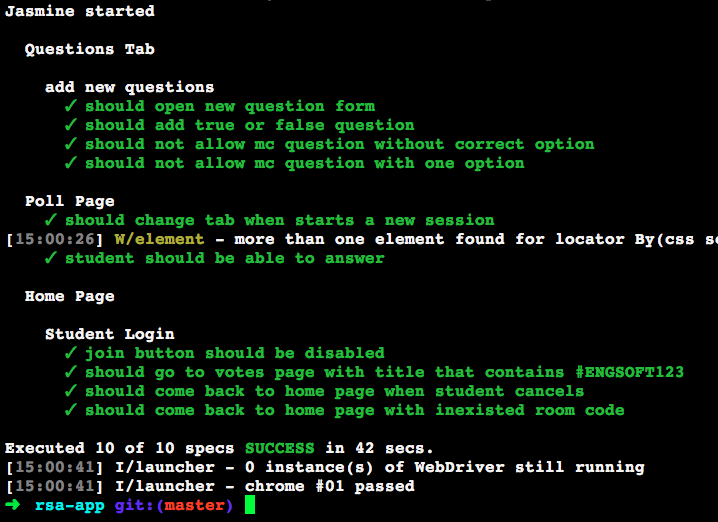
\includegraphics[scale=0.6,valign=t]{imagens/jasmine_test}
  \doautor
\end{figure}

% \afterpage{\clearpage}
\clearpage

\section{Teste de Usabilidade}

Um dos requisitos do software apresentado na \autoref{sec:requisitos} era que:
\begin{description}
\item[Facilidade do uso e de criação de votação:] O sistema não deve oferecer
dificuldades de uso e de criação de questões;
\end{description}

Ou seja, trata-se um de um requisito não funcional do tipo produto (requisitos que
especificam o comportamento do produto), mais especificamente um requisito de usabilidade.
A usabilidade propõe-se a garantir que o produto seja fácil de aprender a usar, eficaz e
agradáveis do ponto de vista do usuário \cite{rogers2013design}.
Para \citeonline{nielsen_2012}, a usabilidade é definida por cinco componentes de qualidade:

\begin{description}
  \item[Apreensiblidade (\textit{Learnability}):] facilidade para os usuários realizarem tarefas básicas
  pela primera vez.
  \item[Eficiência (\textit{Efficiency}):] rapidez com que os usuários realizam uma tarefa, uma vez aprendida.
  \item[Recordação (\textit{Memorability}):] facilidade em lembrar como fazer algo novamente, depois de um período sem uso.
  \item[Erros (\textit{Errors}):] o sistema deve ter uma baixa taxa de erros e ter capacidade de
  recuperação dos erros.
  \item[Satisfação (\textit{Satisfaction}):] quão agradável é utilizar o sistema.
\end{description}

\subsection{Métodos, tarefas e usuários}

Para verificar a usabilidade do software desenvolvido, realizou-se testes de usabilidade, com o
objetivo de testar o quão usável é o software. Para isso, utilizou-se o seguinte método: teste de usabilidade
que incluia a observação dos usuário utilizando o software e também a gravação em vídeo da tela do
software. Além disso, um questionário de satisfação SUS\nomenclature{SUS}{System Usability Scale} (\textit{System Usability Scale}) do usuário foi utilizado para descobrir como
os usuários se sentiram usando o software.

\subsubsection{Questionário de satisfação: SUS}\label{sub:sus}

O SUS é um método normalizado desenvolvido em 1986 por John Brooke.
Ele é um questionário constituído por apenas 10 itens, gratuito e simples de usar.
Utiliza-se a escala de Likert (valores 1 - \textit{discordo totalmente} e 5 \textit{concordo totalmente})
O critérios que o SUS ajuda a avaliar são \cite{brooke1996sus}:

\begin{description}
  \item[Efetividade (\textit{effectiveness})] a capacidade dos usuários de completar tarefas.
  \item[Eficiência (\textit{efficiency})] o nível de esforço e recursos necessários completar as tarefas.
  \item[Satisfação (\textit{satisfaction})] reações subjetivas dos usuários (a experiência foi satisfatória?).
\end{description}

O questionário SUS foi originalmente escrito na língua inglesa. Dessa forma, a versão para língua portuguesa
utilizada nesse trabalho (disponível no \autoref{appendix:sus}) foi a desenvolvida por \citeonline{tenorio2010desenvolvimento} que passou por um processo
de tradução.

O resultado do SUS é a soma individual de cada item, resultando em um número entre 0 e 100.
Para os itens 1, 3, 5, 7 e 9 deve-se subtrair 1 de cada resposta. Para os itens 2, 4, 6, 8 e 10 deve-se
subrair de 5 o valor de cada resposta. O escore final SUS é soma de todos os itens múltiplicada por 2,5 \cite{brooke1996sus}.

\subsubsection{Tarefas}

As tarefas foram desenvolvidas de modo a permitir que os participantes
percorressem todo o processo para permitir disponibilizar as questões para os alunos,
consistindo basicamente nas seguintes tarefas: cadastrar uma turma e alunos, criar questões, iniciar uma sessão de questões,
e controlar a sessão de questões. As tarefas foram escritas no seguinte formato:

\begin{description}
  \item[Título:] em poucas palavras o objetivo da tarefa.
  \item[Descrição:] contexto da tarefa (situação para realizar a tarefa).
  \item[Tarefas:] o que o participante deveria fazer.
\end{description}

O exemplo da \autoref{fig:usabilidade_teste} exibe uma tarefa apresentada para
os participantes seguindo o formato apresentado. A lista completa das tarefas
utilizadas no teste está disponível no \autoref{appendix:tasks}.

\begin{figure}[!ht]
  \centering
  \caption{Exemplo de uma tarefa do teste de usabiliade}
  \label{fig:usabilidade_teste}
  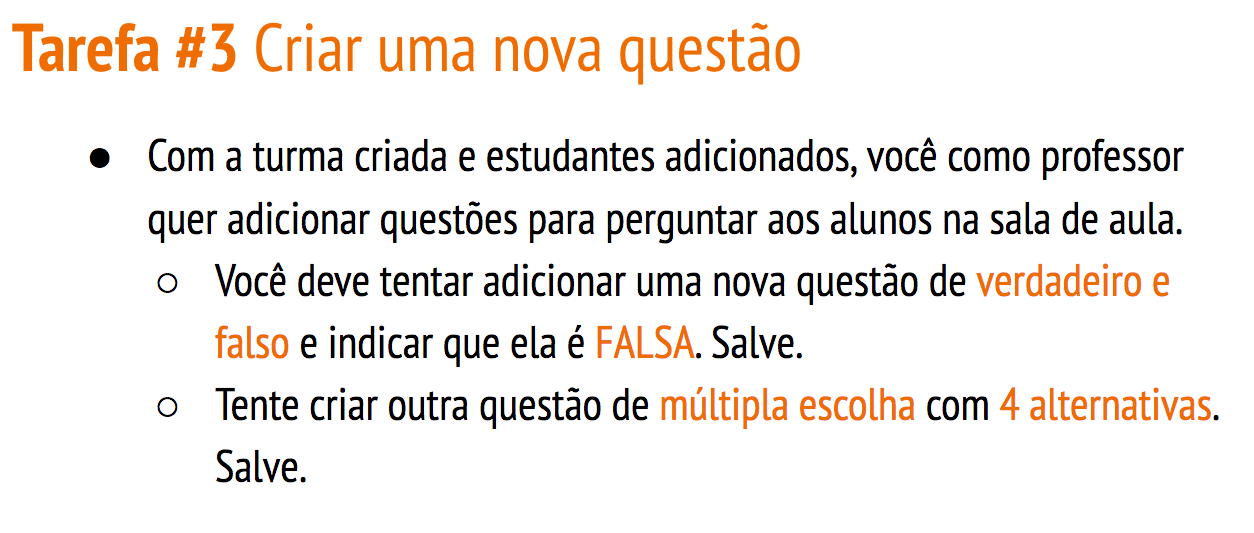
\includegraphics[scale=0.20]{imagens/usability_task}
  \doautor
\end{figure}
\clearpage

A seguir, apresenta-se quais ações eram pretendidas dos participantes em cada tarefa:
\begin{enumerate}[label={},leftmargin=*]
  \item \textbf{Tarefa \#1 Criar uma nova turma}
  \begin{itemize}
    \item Espera-se que o professor identifique facilmente a opção para adicionar uma turma e habilite
    a opção para ativar a turma que ele criou.
  \end{itemize}

  \item \textbf{Tarefa \#2 Adicionar estudantes em uma turma}
  \begin{itemize}
    \item Espera-se que o professor identifique o botão para adicionar estudantes. Na tela de adicionar
    estudantes, que ele identifique a opção \textit{Adicionar manualmente}, adicione os estudantes e em seguida
    salve as alterações.
  \end{itemize}

  \item \textbf{Tarefa \#3 Criar uma nova questão}
  \begin{itemize}
    \item Espera-se que o professor localize a aba \textit{Questões} e identifique facilmente
    o botão para adicionar uma questão. No formulário para adicionar uma questão, que ele
    adicione a pergunta, alternativas e marque uma opção como correta.
  \end{itemize}

  \item \textbf{Tarefa \#4 Realizar frequência dos estudantes}
  \begin{itemize}
    \item Nessa tarefa, o botão de frequência está na aba \textit{Aula}. Seguindo as tarefas de forma
    sequencial, o professor estará na aba \textit{Questões}. Nesse sentido, espera-se
    que o professor explore a aba \textit{Aula} e identifique o botão \textit{Frequência}.
  \end{itemize}

  \item \textbf{Tarefa \#5 Acessar a sala como estudante}
  \begin{itemize}
    \item Agora no papel de aluno, espera-se que o professor relacione o código da turma que
    ele criou na tarefa 1 para ter acesso como estudante no aplicativo. Na tela de identificação do estudante,
    espera-se que ao ler a mensagem ele coloque o código de identificação de um estudante adicionado na tarefa 2.
  \end{itemize}

  \item \textbf{Tarefa \#6 Responder a frequência}
  \begin{itemize}
    \item Já identificado no aplicativo do estudante, espera-se que o professor identifique
    o botão \textit{Responder chamada} e entre com o código gerado para a frequência na tarefa 4.
    Por último, espera-se que ele verifique que no software do professor, o sistema identificou
    que um aluno realizou a frequência.
  \end{itemize}

  \item \textbf{Tarefa \#7 Iniciar sessão de perguntas}
  \begin{itemize}
    \item  Espera-se que o professor navegue para a aba \textit{Questões} e identifique
    que para iniciar uma sessão de perguntas, ele deve selecionar pelo menos uma questão que ele criou
    na tarefa 3. Ele também deve explorar as opções de controle da sessão e ativar uma questão para votação.
  \end{itemize}

  \item \textbf{Tarefa \#8 Responder questão}
  \begin{itemize}
    \item Com a questão já ativada, o professor deve facilmente escolher uma alternativa e
    enviar a resposta utilizando o aplicativo do estudante.
  \end{itemize}

  \item \textbf{Tarefa \#9 Finalizar sessão de perguntas}
  \begin{itemize}
    \item Espera-se que o professor explore as opções de pausar, mostrar a resposta correta e mostrar
    o resultado da votação.
  \end{itemize}

  \item \textbf{Tarefa \#10 Encerrar sessão de perguntas}
  \begin{itemize}
    \item Espera-se que o professor identifique a opção de encerrar a sessão de perguntas.
  \end{itemize}

  \item \textbf{Tarefa \#11 Verificar resposta dos estudantes}
  \begin{itemize}
    \item Encerrando a sessão de perguntas, a sessão encerrada deve ser listada no software.
    Espera-se que o professor clique na opção detalhes da sessão listada e explore as respostas dos estudantes.
  \end{itemize}
\end{enumerate}

\subsubsection{Usuários}

Os participantes foram considerados usuários típicos, 4 professores da UNIVASF e
um estudante de graduação de que já trabalhou como professor do ensino médio. Todos os
participantes eram do sexo masculino.

\subsection{Resultado e discussões}

Com a utilização do questionário SUS foi possível mensurar o grau de satisfação quanto
a usabilidade do software desenvolvido. Além disso, ele permite avaliar os componentes da
qualidade indicadas por \citeonline{nielsen_2012} distribduídas nas afirmativas do questionário:

\begin{itemize}
  \item \textbf{Apreensiblidade}: afirmações 3, 4, 7 e 10:
  \begin{itemize}
    \item AF3: Eu achei o sistema fácil de usar.
    \item AF4: Eu acho que precisaria de ajuda de uma pessoa com conhecimentos
    técnicos para usar o sistema
    \item AF7: Eu imagino que as pessoas aprenderão como usar esse sistema
    rapidamente.
    \item AF10: Eu precisei aprender várias coisas novas antes de conseguir
    usar o sistema.
  \end{itemize}
  \item \textbf{Eficiência}: afirmações 5, 6 e 8:
  \begin{itemize}
    \item AF5: Eu acho que as várias funções do sistema estão muito bem
    integradas.
    \item AF6: Eu acho que o sistema apresenta muita inconsistência.
    \item AF8: Eu achei o sistema atrapalhado de usar.
  \end{itemize}
  \item \textbf{Recordação}: afirmação 2:
  \begin{itemize}
    \item AF2: Eu acho o sistema desnecessariamente complexo.
  \end{itemize}
  \item \textbf{Erros}: afirmação 6:
  \begin{itemize}
    \item AF6: Eu acho que o sistema apresenta muita inconsistência.
  \end{itemize}
  \item \textbf{Satisfação}: afirmações 1, 4 e 9:
  \begin{itemize}
    \item AF1: Eu acho que gostaria de usar esse sistema frequentemente.
    \item AF4: Eu acho que precisaria de ajuda de uma pessoa com conhecimentos
    técnicos para usar o sistema.
    \item AF9: Eu me senti confiante ao usar o sistema.
  \end{itemize}
\end{itemize}

A \autoref{tab:sus_result} apresenta as respostas dos 5 participantes no teste de usabilidade.
A coluna \textit{Afirmações} contém as afirmações do questionário SUS, seguida pelas colunas
\textit{P1,$\ldots$,P5}, que representam cada participante. Os valores da escala de Likert
(1 - discordo totalmente e 5 - concordo plenamente) escolhidas pelos participantes estão mostradas
na tabela.

Abaixo das afirmações apresenta-se a \textit{Pontuação SUS} de cada questionário. O cálculo
para obter tais resultados foi apresentado na \autoref{sub:sus}. Obteve-se uma média de
85,50 com desvio padrão de 9,42.

A \autoref{fig:sus_score} apresenta como alguns estudos classificam a nota média do SUS.
Dessa forma, o software pode ser classificado como \textit{80-90, aceitável, B e Excelente}.
Assim, pode-se dizer que o software apresenta os cinco componentes de qualidade de usabilidade definidos
por \citeonline{nielsen_2012}, ou seja, apreensibilidade, eficiência, recordação, erros e satisfação
de forma excelente.

\begin{figure}[!ht]
  \centering
  \caption{Resultado do questionário SUS}
  \label{tab:sus_result}
\begin{tabular}{>{\raggedright}p{0.45\paperwidth}||ccccc}
\hline
\multicolumn{6}{c}{\textbf{Resultado do questionário SUS}}\tabularnewline
\hline
\hline
\multirow{2}{0.5\paperwidth}{\centering{}\textbf{Afirmações}} & \multicolumn{5}{c}{Participantes}\tabularnewline
 & P1 & P2 & P3 & P4 & P5\tabularnewline
\hline
\hline
\textbf{AF1} - {\small{}Eu acho que gostaria de usar esse sistema frequentemente.}
 & 5 & 4 & 4 & 4 & 5\tabularnewline
\textbf{AF2} - {\small{}Eu acho o sistema desnecessariamente complexo.}
 & 4 & 1 & 2 & 2 & 1\tabularnewline
\textbf{AF3} - {\small{}Eu achei o sistema fácil de usar.}
 & 4 & 5 & 3 & 4 & 5\tabularnewline
\textbf{AF4} - {\small{}Eu acho que precisaria de ajuda de uma pessoa com conhecimentos
técnicos para usar o sistema.}
 & 1 & 1 & 4 & 4 & 2\tabularnewline
\textbf{AF5} - {\small{}Eu acho que as várias funções do sistema estão muito bem
integradas.}
 & 4 & 5 & 5 & 4 & 4\tabularnewline
\textbf{AF6} - {\small{}Eu acho que o sistema apresenta muita inconsistência.}
 & 2 & 1 & 1 & 1 & 1\tabularnewline
\textbf{AF7} - {\small{}Eu imagino que as pessoas aprenderão como usar esse sistema
rapidamente.}
 & 5 & 5 & 4 & 4 & 5\tabularnewline
\textbf{AF8} - {\small{}Eu achei o sistema atrapalhado de usar.}
 & 1 & 1 & 1 & 2 & 1\tabularnewline
\textbf{AF9} - {\small{}Eu me senti confiante ao usar o sistema.}
 & 5 & 4 & 4 & 5 & 5\tabularnewline
\textbf{AF10} - {\small{}Eu precisei aprender várias coisas novas antes de conseguir
usar o sistema.}
 & 1 & 2 & 2 & 1 & 1\tabularnewline
\hline
\centering{}\textbf{Pontuação SUS} & 85 & 95 & 75 & 77,5 & 95\tabularnewline
\hline
\end{tabular}
\doautor
\end{figure}

\begin{figure}[!ht]
  \centering
  \caption{Comparação das classificações adjetivas, pontuações de aceitabilidade e escalas de classificação escolar, em relação ao escore médio do SUS}
  \label{fig:sus_score}
  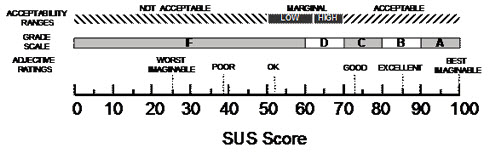
\includegraphics[scale=1.5]{imagens/sus_score}
  \fonte{\cite{bangor2009determining}}
\end{figure}

\clearpage
\subsubsection{Análise das gravações por tarefa}
Para cada uma das tarefas propostas, as principais observações de cada tarefa
estão descritas a seguir:

\begin{enumerate}[label={},leftmargin=*]
  \item \textbf{Tarefa \#1 Criar uma nova turma}
  \begin{description}
    \item [Expectativa:] Espera-se que o professor identifique facilmente a opção para adicionar uma turma e habilite
    a opção para ativar a turma que ele criou.
    \item [Observações:] Todos os participantes conseguiram concluir essa tarefa sem ajuda. O botão
    para adicionar a turma foi identificado com facilidade. 1 participante não ativou a turma.
    \item [Melhorias:] Quando nenhuma turma estiver ativada, exibir uma mensagem indicando:
    \textit{Você ainda não tem uma turma ativada. Ative uma turma para iniciar uma sessão de perguntas}.
    Outra solução seria ativar a primeira turma criada automaticamente e exibir uma mensagem para o usuário.
  \end{description}

  \item \textbf{Tarefa \#2 Adicionar estudantes em uma turma}
  \begin{description}
    \item [Esperado:] Espera-se que o professor identifique o botão para adicionar estudantes. Na tela de adicionar
    estudantes, que ele identifique a opção \textit{Adicionar manualmente}, adicione os estudantes e em seguida
    salve as alterações.
    \item [Observações:] 2 participantes tiveram dificuldades para encontrar o botão para
    adicionar estudantes no canto inferior direito da tela.
    \item [Solução:] Quando a lista de estudantes estiver vazia, exibir uma mensagem indicando:
    \textit{Você ainda não tem nenhum estudante cadastrado na turma. Começe adicionando estudantes nas opções ao lado.}
  \end{description}

  \item \textbf{Tarefa \#3 Criar uma nova questão}
  \begin{description}
    \item [Esperado:] Espera-se que o professor localize a aba \textit{Questões} e identifique facilmente
    o botão para adicionar uma questão. No formulário para adicionar uma questão, que ele
    adicione a pergunta, alternativas e marque uma opção como correta.
    \item[Observações:] Todos os participantes concluíram essa tarefa sem ajuda. 2 participantes
    tiveram um pouco de dificuldade para marcar uma alternativa como correta.
    \item[Melhorias:]
    Colocar a descrição \textit{Correta} ao lado do botão que seleciona a questão como correta.
    Outra melhoria seria que quando o tipo de questão for de múltipla escolha, já adicionar
    duas alternativas como padrão, diminuindo assim dois cliques no processo.
  \end{description}

  \item \textbf{Tarefa \#5 Acessar a sala como estudante}
  \begin{description}
    \item [Esperado:] Agora no papel de aluno, espera-se que o professor relacione o código da turma que
    ele criou na tarefa 1 para ter acesso como estudante no aplicativo. Na tela de identificação do estudante,
    espera-se que ao ler a mensagem ele coloque o código de identificação de um estudante adicionado na tarefa 2.
    \item [Observações:] 1 participante precisou de ajuda para completar a tarefa. Uma observação de um
    participante foi que ele estava precisando digitar o código da turma a todo instante.
    \item [Melhorias:] Quando um estudante entrar em uma turma com um código de acesso, o sistema
    deve guardar o código em uma lista de acessos recentes para facilitar os acessos futuros.
  \end{description}

  \item \textbf{Tarefa \#7 Iniciar sessão de perguntas}
  \begin{description}
    \item[Esperado:]  Espera-se que o professor navegue para a aba \textit{Questões} e identifique
    que para iniciar uma sessão de perguntas, ele deve selecionar pelo menos uma questão que ele criou
    na tarefa 3. Ele também deve explorar as opções de controle da sessão e ativar uma questão para votação.
    \item[Observações:] 3 participantes pediram ajuda para completar essa tarefa. Percebeu-se que
    na aba \textit{Aula}, era exibido o aviso - \textit{Nenhuma sessão encerrada}, fazendo
    com que o usuário entende-se que uma sessão deveria ser iniciada em algum lugar na aba \textit{Aula}, já que
    a mesma fazia referência as sessões encerradas.
    \item[Melhorias:] Na aba \textit{Aula} quando um aviso indicando que:
    \textit{Para iniciar uma sessão, na aba QUESTÕES selecione uma ou mais questões e clique em INICIAR SESSÃO}.
    Na aba \textit{Questões}, quando o professor clicar no botão \textit{INICIAR SESSÃO} sem nenhuma
    questão selecionada, deve aparecer uma mensagem indicando: \textit{Selecione uma ou mais questões para iniciar uma sessão}.
  \end{description}

  \item \textbf{Tarefas \#4, 6, 8, 9, 10 e 11}
  \begin{description}
    \item [Observação:] Todos os participantes concluíram essas tarefas com sucesso e sem ajuda.
  \end{description}
\end{enumerate}

\section{Teste em Sala de Aula}

O teste de usabilidade descrito nas seções anteriores, pode-se classificá-lo além de um teste de usabilidade,
também como um teste alpha. \citeonline{Pressman2009} define o teste alpha como um teste
conduzido pelo usuário ou cliente no ambiente do desenvolvedor, este observando
o usuário, registrando erros e problemas de uso.

O teste de usabilidade foi conduzido em um ambiente definido pelo desenvolvedor, este controlando
todas as variáveis do ambiente (internet, computador, celular, etc), capturando as ações do usuário e
fazendo anotações sobre o comportamento, vozes, etc.

Quando um software é testado em um ambiente não controlado pelo desenvolvedor,
chama-se esse teste de \textit{teste beta}. Para \citeonline{Pressman2009}, o teste beta é aquele em
que uma versão do software é disponibilizado aos usuários para que possam experimentar e
eventualmente levantar os problemas encontrados com os desenvolvedores.

Realizamos um teste beta para testar funcionamento do aplicativo do estudante em diferentes
\textit{smartphones} e/ou computadores e o uso do software do professor na sala de aula.
Para isso, uma versão do sistema operacional Android do aplicativo foi gerada e disponibilizada na
loja na loja online da Google para distribuição de aplicações, Google Play\footnote{Endereço do aplicativo no Google Play: \href{https://play.google.com/store/apps/details?id=apps.pedrosobral.rsa}{play.google.com/store/apps/details?id=apps.pedrosobral.rsa}}.
Dessa forma, tanto o professor quanto os estudantes poderam instalar o aplicativo nos seus aparelhos.

\subsection{Participantes}

O teste foi realizado na disciplina \textit{Modelagem e Simulação} do curso de graduação
em Engenharia de Computação da Universidade Federal do Vale do São Francisco (UNIVASF).
O objetivo geral dessa disciplina é ``tornar os alunos capazes de construir sistemas de
simulação, de validar e verificar os modelos, e de validar os resultados da simulação'' \cite{ppcComputacao}.
O teste foi realizado no dia 19 de julho de 2017, no campus Juazeiro - BA.

A turma era composta por um professor e 13 alunos, com faixa etária entre 20 e 27 anos, 3 (23\%)
alunos do sexo feminino e 10 (74\%) alunos do sexo masculino. Todos os estudantes
tinham acesso a um \textit{smartphone}, 12 (92\%) do sistema operacional Android e um
1 (8\%) do sistema operacional Windows Phone.
Nenhum deles havia utilizado um aplicativo de sistema de resposta na sala de aula anteriormente.

\subsection{Procedimento}

O professor da disciplina anteriormente ao teste na sala de aula, participou do teste de usabilidade,
dessa forma ele já tinha os conhecimentos básicos do software. Ele também foi responsável por criar
as questões no aplicativo que foram apresentadas aos estudantes na sala de aula.
